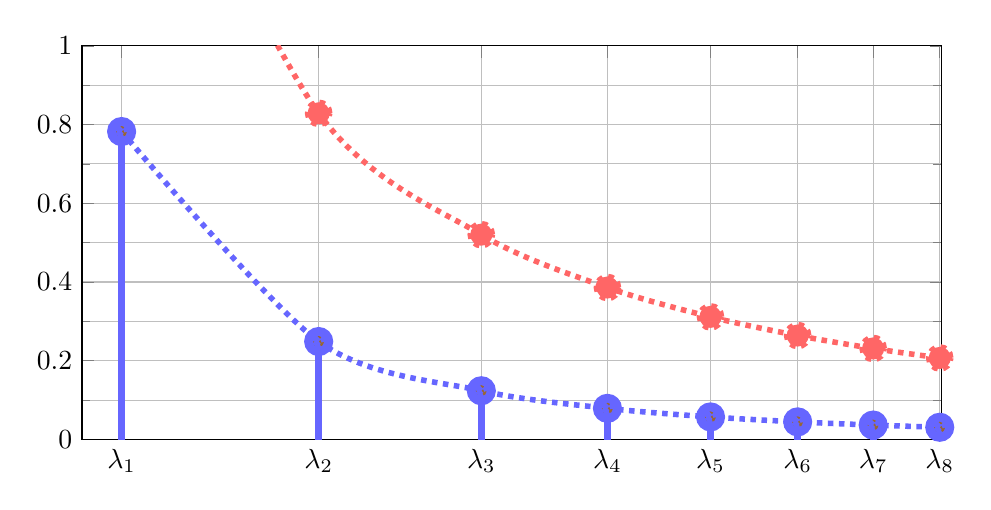
\begin{tikzpicture}
\begin{axis}[
    xlabel={},
    ylabel={},
    ymin=0, ymax=1, % Adjust according to the actual range of your data
    xmin=0.68, xmax=2.2,
    scale only axis,
     xtick = { 0., 0.75,  1.09861229,  1.38629436, 1.60943791, 1.79175947, 1.94591015, 2.07944154, 2.19722458},
     xticklabels = {$\lambda_1$,
     $\lambda_1$,
     $\lambda_2$,
     $\lambda_3$,
     $\lambda_4$,
     $\lambda_5$,
     $\lambda_6$,
     $\lambda_7$,
     $\lambda_8$,},
    samples at={0., 0.75, 1.09861229, 1.38629436, 1.60943791,
       1.79175947, 1.94591015, 2.07944154, 2.19722458},
    grid=both,
    minor tick num=1,
    every axis plot/.append style={thick},
    height = 5cm,
    width = .9\linewidth
]

% Stem plot with markers explicitly defined
\addplot+[ycomb, mark=*, blue!60, mark options={fill=blue!60, scale=2}, line width   = 2.5] plot (x, {.33/(x^3});
% Dotted line plot
\addplot+[smooth, mark=*, red!60, mark options={fill=red!60, scale=2}, line width   = 2, dotted] expression {1/(x^2};

\addplot+[smooth, blue!60, line width   = 2, dotted] expression {.33/(x^3};

\end{axis}
\end{tikzpicture}